% Classe default, de acordo com o modelo:
\documentclass[12pt,a4paper,openright,titlepage,oneside]{book}

% Classe alternativa, apropriada para impressão frente-verso. Inclui páginas em branco
% de forma que capítulos sempre tenham início na página à direita:
% \documentclass[11pt,a4paper,openright,titlepage]{book}

% Pacotes
\usepackage[T1]{fontenc}
\usepackage[utf8]{inputenc}
\usepackage[brazilian]{babel}
\usepackage{epsfig}
\usepackage{subfigure}
\usepackage{amsfonts}
\usepackage{amsmath,mathrsfs}
\usepackage{amssymb}
\usepackage[thmmarks,amsmath]{ntheorem}%\usepackage{amsthm}
\usepackage{boxedminipage}
\usepackage{geometry}
\usepackage{theorem}
\usepackage{fancybox}
\usepackage{fancyhdr}
\usepackage{ifthen}
\usepackage{url}
\usepackage{afterpage}
\usepackage{color}
\usepackage{colortbl}
\usepackage{rotating}
\usepackage{makeidx}
\usepackage{epstopdf}
\usepackage{indentfirst}
\usepackage[pdfstartview=FitH]{hyperref}
\usepackage[table,xcdraw]{xcolor}
\usepackage{multirow}
\usepackage{pdfpages}
\usepackage{lastpage}
\usepackage{enumerate}

%pacote para usar o comando \widebar{}
\usepackage{mathabx}
%frames para notas
\usepackage[framemethod=default]{mdframed}


\usepackage[thinlines]{easytable}
%configuracao de legendas para figuras e graficos
\usepackage[labelfont=small,textfont={small,it}]{caption}

%secao para codigos
\usepackage[framed,numbered,autolinebreaks,useliterate]{mcode}

%mudança na formatacao de paragrafos

\usepackage{titlesec}
\setcounter{secnumdepth}{4}

\titleformat{\paragraph}
{\normalfont\normalsize\bfseries}{\theparagraph}{1em}{}
\titlespacing*{\paragraph}
{0pt}{3.25ex plus 1ex minus .2ex}{1.5ex plus .2ex}




%----------------------------------------comandos para enunciar e enumerar enunciados
\newcommand{\dem}{\quad {\bf Demonstração:}\quad}
\newcommand{\fim}{\newline \begin{flushright} $\blacksquare$ \end{flushright}}
\newtheorem{defi}{Definição}[section]
\newtheorem{lema}{Lema}[section]
\newtheorem{conj}{Conjectura}[section]
\newtheorem{exem}{Exemplo}[section]
\newtheorem{axi}{Axioma}[section]
\newtheorem{prop}{Propriedade}[section]
\newtheorem{obs}{Observação}[section]
\newtheorem{teo}{Teorema}[section]
\newtheorem{corol}{Corolário}[section]
\newtheorem{res}{Resolução}[section]
%----------------------------------------------sí­mbolos
\newcommand{\R}{\mathbb{R}}%reais
\newcommand{\dotp}{\bullet}%produto escalar
\newcommand{\K}{\mathbb{K}}%corpo qualquer
\newcommand{\C}{\mathbb{C}}%complexos
\newcommand{\N}{\mathbb{N}}%naturais
\newcommand{\Z}{\mathbb{Z}}%inteiros
\newcommand{\Q}{\mathbb{Q}}%racionais
\newcommand{\U}{\mathcal{U}}%espaços vetoriais
\newcommand{\V}{\mathcal{V}}%espaços vetoriais
\newcommand{\W}{\mathcal{W}}%espaços vetoriais
\newcommand{\E}{\mathbb{E}}%espaços vetoriais
\newcommand{\HRule}{\rule{\linewidth}{0.5mm}}
\newcommand{\X}{$\bullet$}
\newcommand{\ignore}[1]{}
\newcommand{\MATLAB}{$\text{MATLAB}^{\text{\textregistered}}$}
%-------------------------------------------------------------------------------------


\global\mdfdefinestyle{exampledefault}{%
	linecolor=lightgray,linewidth=1pt,%
	leftmargin=1cm,rightmargin=1cm,
}


%\usepackage[pdftex,a5paper,%
%pdftitle={The Ducks},%
%pdfauthor={Mother Goose},%
%colorlinks=true,%
%linkcolor=blue%
%]
\usepackage[framed,numbered]{config/mcode}
%\lstinputlisting{/path_to_mfile/yourmfile.m}
\hypersetup{colorlinks,%
citecolor=black,%
filecolor=black,%
linkcolor=black,%
urlcolor=black
}
\usepackage{array}
\usepackage{tabularx}
\usepackage{caption} 
%\captionsetup[table]{skip=10pt}
\newcolumntype{C}[1]{>{\centering\let\newline\\\arraybackslash\hspace{0pt}}m{#1}}
\newcolumntype{L}[1]{>{\raggedright\let\newline\\\arraybackslash\hspace{0pt}}m{#1}}
\newcolumntype{R}[1]{>{\raggedleft\let\newline\\\arraybackslash\hspace{0pt}}m{#1}}
\usepackage[font=small]{caption}
\usepackage{lastpage}
% Escolher um dos seguintes formatos:
\usepackage{config/ft_unb} % segue padrão de fonte Times
%\usepackage[num,abnt-etal-list=0]{config/abntex2/abntex2cite} % Citações pela ABNT
\usepackage[alf,abnt-etal-list=0]{config/abntex2/abntex2cite}

\newcommand{\citeC}[1]{[\citeonline{#1}]}
\renewcommand{\labelitemi}{$-$}


% Ambiente para inserir notas no meio do texto
\newenvironment{mymdframed}[1]{%
	\mdfsetup{%
		frametitle={\colorbox{white}{\,#1\,}},
		frametitleaboveskip=-\ht\strutbox,
		frametitlealignment=\raggedright
	}%
\begin{mdframed}[style=exampledefault]
}{\end{mdframed}}


\makeindex
 
%%%%%%%%%%%%%%%%%%%%%%%%%%%%%%%%%%%%%%%%%%%%%%%%%%%%%%%%%%%%%%%%%%%%%%%%%
% Compilações parciais: com o comando abaixo, selecione apenas os capitulos
% que deseja compilar. Por exemplo, veja o que acontece se descomentar a
% linha abaixo:
% \includeonly{resumos}
%%%%%%%%%%%%%%%%%%%%%%%%%%%%%%%%%%%%%%%%%%%%%%%%%%%%%%%%%%%%%%%%%%%%%%%%%

%%%%%%%%%%%%%%%%%%%%%%%%%%%%%%%%%%%%%%%%%%%%%%%%%%%%%%%%%%%%%%%%%%%%%%%%%
% Documento principal													%
%%%%%%%%%%%%%%%%%%%%%%%%%%%%%%%%%%%%%%%%%%%%%%%%%%%%%%%%%%%%%%%%%%%%%%%%%
\begin{document}

\setcounter{secnumdepth}{3} % numeração de seções até nível 3
\setcounter{tocdepth}{2} % numeração de seções no sumário até nível 2
\pagestyle{empty}

%%%%%%%%%%%%%%%%%%%%%%%%%%%%%%%%%%%%%%%%%%%%%%%%%%%%%%%%%%%%%%%%%%%%%%%%%
% GRAU PRETENDIDO E TIPO DE MONOGRAFIA									%
%%%%%%%%%%%%%%%%%%%%%%%%%%%%%%%%%%%%%%%%%%%%%%%%%%%%%%%%%%%%%%%%%%%%%%%%%
% Alguns exemplos seguem abaixo. Se o seu for algum deles, descomente-o. Em geral, o grau e o tipo de monografia associado estão na mesma linha.
%\grau{Título}{especificação} \tipodemonografia{"a" para feminino e "e" para masculino}{Tipo}
%\grau{Doutor}{em Engenharia Elétrica} \tipodemonografia{a}{Tese de Doutorado}
%\grau{Mestre}{em Engenharia de Sistemas Eletrônicos e Automação} \tipodemonografia{a}{Dissertação de Mestrado}
\grau{Engenheiro}{Eletricista} \tipodemonografia{o}{Trabalho de Conclusão de Curso}

%%%%%%%%%%%%%%%%%%%%%%%%%%%%%%%%%%%%%%%%%%%%%%%%%%%%%%%%%%%%%%%%%%%%%%%%%
% TÍTULO																%
%%%%%%%%%%%%%%%%%%%%%%%%%%%%%%%%%%%%%%%%%%%%%%%%%%%%%%%%%%%%%%%%%%%%%%%%%
% Os comandos a seguir servem para definir o título do trabalho. Para evitar  que o latex defina automaticamente a quebra de linha, foram definidos um comando por linha. Desta forma o autor define como quer que o título seja dividio em várias linhas. O exemplo abaixo é para um título que ocupa três linhas. Observe que mesmo com a linha 4 não sendo utilizada, o comando \titulolinhaiv é chamado.
\titulolinhai{Tratamento de Sinal de Áudio}
\titulolinhaii{com aplicações em Música Digital}
\titulolinhaiii{\textit{Reverb Shimmer}}
\titulolinhaiv{}

%%%%%%%%%%%%%%%%%%%%%%%%%%%%%%%%%%%%%%%%%%%%%%%%%%%%%%%%%%%%%%%%%%%%%%%%%
% AUTORES																%
%%%%%%%%%%%%%%%%%%%%%%%%%%%%%%%%%%%%%%%%%%%%%%%%%%%%%%%%%%%%%%%%%%%%%%%%%
% Os nomes dos autores são definidos pelos comandos \autori (autor 1) e \autorii (autor 2). Para trabalhos com apenas um autor, deve-se usar \autorii{} para que não apareça um nome para segundo autor.
\autori{Filipe Miguel Ribeiro}
\autorii{Nome do Autor 2}
\autorii{} % descomente esta linha se não houver segundo autor.
\autoriii{Nome do Autor 3}
\autoriii{} % descomente esta linha se não houver terceiro autor.

%%%%%%%%%%%%%%%%%%%%%%%%%%%%%%%%%%%%%%%%%%%%%%%%%%%%%%%%%%%%%%%%%%%%%%%%%
% BANCA EXAMINADORA														%
%%%%%%%%%%%%%%%%%%%%%%%%%%%%%%%%%%%%%%%%%%%%%%%%%%%%%%%%%%%%%%%%%%%%%%%%%
% Os nomes dos membros da banca são definidos a seguir. Pode-se ter até 5 membros da banca, numerados de i a v (algarismos romanos).
% Para trabalhos com apenas um autor, deve-se usar \autorii{} para que não apareça um nome para segundo autor. É incubência do usuário definir no argumento dos comandos a afiliação do membro da banca, assim como sua posição (se for orientador ou co-orientador). 
% Os nomes definidos pelos comandos abaixo aparecem na ordem de i a v.
\membrodabancai{Prof. Dr. André Café, ENE/UnB}
\membrodabancaifuncao{Orientador}
\membrodabancaii{Prof. Fulano de Tal 2, ENE/UnB}
\membrodabancaiifuncao{Examinador Interno}
\membrodabancaiii{Prof. Fulano de Tal 2, ENE/UnB}
\membrodabancaiiifuncao{Examinador interno}
\membrodabancaiv{Prof. Fulano de Tal 2, ENE/UnB}
\membrodabancaivfuncao{Examinador interno}
\membrodabancav{}
\membrodabancavfuncao{}

%%%%%%%%%%%%%%%%%%%%%%%%%%%%%%%%%%%%%%%%%%%%%%%%%%%%%%%%%%%%%%%%%%%%%%%%%
% DATA DA DEFESA														%
%%%%%%%%%%%%%%%%%%%%%%%%%%%%%%%%%%%%%%%%%%%%%%%%%%%%%%%%%%%%%%%%%%%%%%%%%
\mes{julho}
\ano{2017}

%%%%%%%%%%%%%%%%%%%%%%%%%%%%%%%%%%%%%%%%%%%%%%%%%%%%%%%%%%%%%%%%%%%%%%%%%
% FICHA CATALOGRÁFICA													%
%%%%%%%%%%%%%%%%%%%%%%%%%%%%%%%%%%%%%%%%%%%%%%%%%%%%%%%%%%%%%%%%%%%%%%%%%
%Colocar o nome do autor como vai aparecer no catálogo. Último sobrenome primeiro, depois o nome e sobrenomes intermediários. Ex.: Borges, Geovany Araújo
\autorcatalogo{Ribeiro, Filipe Miguel}
%Colocar o nome abreviado. Último sobrenome primeiro, depois as iniciais do nome e sobrenomes intermediários. Ex.: Borges, G.A.
\autorabreviadocatalogo{Ribeiro, F. M.}

%%%%%%%%%%%%%%%%%%%%%%%%%%%%%%%%%%%%%%%%%%%%%%%%%%%%%%%%%%%%%%%%%%%%%%%%%
% PALAVRAS CHAVE														%
%%%%%%%%%%%%%%%%%%%%%%%%%%%%%%%%%%%%%%%%%%%%%%%%%%%%%%%%%%%%%%%%%%%%%%%%%
\palavraschavecatalogoi{Efeito Reverb Shimmer}
\palavraschavecatalogoii{Microntrolador MSP430}
\palavraschavecatalogoiii{Misturas Convolutivas}
\palavraschavecatalogoiv{Separação de sinais de fala}

%%%%%%%%%%%%%%%%%%%%%%%%%%%%%%%%%%%%%%%%%%%%%%%%%%%%%%%%%%%%%%%%%%%%%%%%%
% NÚMERO DA PUBLICAÇÃO													%
%%%%%%%%%%%%%%%%%%%%%%%%%%%%%%%%%%%%%%%%%%%%%%%%%%%%%%%%%%%%%%%%%%%%%%%%%
%fornecido pelo departamento após a defesa
%\publicacao{TCC-}

%Número de páginas da dissertação.
\numeropaginascatalogo{\pageref{LastPage}~p.}

% Comandos para criar a capa e a página de assinaturas.
\capaprincipal
\capaassinaturas
\setcounter{page}{3}

% Comando para criar a ficha catalográfica
\fichacatalografica

\frontmatter
\fontsize{12}{14}\selectfont

% Comando para criar a página de dedicatória
%%%%%%%%%%%%%%%%%%%%%%%%%%%%%%%%%%%%%%%%%%%%%%%%%%%%%%%%%%%%%%%%%%%%%%%%%
% Dedicatória															%
%%%%%%%%%%%%%%%%%%%%%%%%%%%%%%%%%%%%%%%%%%%%%%%%%%%%%%%%%%%%%%%%%%%%%%%%%
% Texto de dedicatória do primeiro autor
\dedicatoriaautori{Dedicatória do autor 1}

% Texto de dedicatória do segundo autor. Caso não tenha um segundo autor, este texto não 
% será mostrado
\dedicatoriaautorii{Dedicatória do autor 2}

% Texto de dedicatória do terceiro autor. Caso não tenha um segundo autor, este texto não 
% será mostrado
\dedicatoriaautoriii{Dedicatória do autor 3}

\dedicatoria

% Comando para criar a página de agradecimentos
%%%%%%%%%%%%%%%%%%%%%%%%%%%%%%%%%%%%%%%%%%%%%%%%%%%%%%%%%%%%%%%%%%%%%%%%%
% Agradecimentos
%%%%%%%%%%%%%%%%%%%%%%%%%%%%%%%%%%%%%%%%%%%%%%%%%%%%%%%%%%%%%%%%%%%%%%%%%
% Texto de agradecimentos do primeiro autor
\agradecimentosautori{A inclusão desta seção de agradecimentos é opcional e fica à critério do(s) autor(es), que caso deseje(em) inclui-la deverá(ao) utilizar este espaço, seguindo está formatação.}

% Texto de agradecimentos do segundo autor. Caso não tenha um segundo autor, este texto não 
% será mostrado
\agradecimentosautorii{A inclusão desta seção de agradecimentos é opcional e fica à critério do(s) autor(es), que caso deseje(em) inclui-la deverá(ao) utilizar este espaço, seguindo está formatação.}

% Texto de agradecimentos do segundo autor. Caso não tenha um terceiro autor, este texto não 
% será mostrado
\agradecimentosautoriii{A inclusão desta seção de agradecimentos é opcional e fica à critério do(s) autor(es), que caso deseje(em) inclui-la deverá(ao) utilizar este espaço, seguindo está formatação.}
\agradecimentos

\setcounter{page}{6}

%TCIDATA{LaTeXparent=0,0,relatorio.tex}

\resumo{Resumo}{INSIRA SEU RESUMO AQUI.}

\vspace*{2cm}

\resumo{Abstract}{INSERT YOUR ABSTRACT HERE.}

%%%%%%%%%%%%%%%%%%%%%%%%%%%%%%%%%%%%%%%%%%%%%%%%%%%%%%%%%%%%%%%%%%%%%%%%%
% Listas de conteúdo, figuras e tabelas.								%
%%%%%%%%%%%%%%%%%%%%%%%%%%%%%%%%%%%%%%%%%%%%%%%%%%%%%%%%%%%%%%%%%%%%%%%%%
\sumario
\listadefiguras
\listadetabelas


%%%%%%%%%%%%%%%%%%%%%%%%%%%%%%%%%%%%%%%%%%%%%%%%%%%%%%%%%%%%%%%%%%%%%%%%%
% Lista de simbolos.													%
%%%%%%%%%%%%%%%%%%%%%%%%%%%%%%%%%%%%%%%%%%%%%%%%%%%%%%%%%%%%%%%%%%%%%%%%%
%\pdfbookmark[level]{text}{}
%TCIDATA{LaTeXparent=0,0,these.tex}
                      

%\chapter*{\setfontarial\mdseries LISTA DE SÍMBOLOS} % se usar ft1unb.sty, descomente esta linha
\chapter*{LISTA DE SÍMBOLOS} % se usar ft2unb.sty, descomente esta linha

\subsection*{Símbolos Latinos}

\begin{tabular}{p{0.1\textwidth}p{0.63\textwidth}>{\PreserveBacklash\raggedleft}p{0.15\textwidth}}
$Q$	& Fluxo	& [ml/s]\\
%$Cp$ & Calor especifico a pressão constante	&  [kJ/kg.K]\\
%$h$	& Entalpia especifica	& [kJ/kg]\\
%$\dot{m}$	& Vazão mássica	& [kg/s]\\
%$T$	& Temperatura	& [$^\circ$C]\\
%$U$	& Coeficiente global de transferência de calor & [W/m$^2$.K]
\end{tabular}
%
\subsection*{Símbolos Gregos}

\begin{tabular}{p{0.1\textwidth}p{0.63\textwidth}>{\PreserveBacklash\raggedleft}p{0.15\textwidth}}

$\Delta$	& Variação entre duas grandezas similares\\
$\varepsilon$ & Fração muito pequena de uma certa grandeza 

\end{tabular}

\subsection*{Grupos Adimensionais}

\begin{tabular}{p{0.1\textwidth}p{0.80\textwidth}}
$e$ &	Número de Euler \\


\end{tabular}

\subsection*{Subscritos}

\begin{tabular}{p{0.1\textwidth}p{0.80\textwidth}}
$max$	& Máximo \\
%$min$	& Mínimo \\

\end{tabular}

\subsection*{Sobrescritos}

\begin{tabular}{p{0.1\textwidth}p{0.80\textwidth}}
%$\cdot$	& Variação temporal \\
$-$	& Valor médio
\end{tabular}

\subsection*{Siglas}

\begin{tabular}{p{0.1\textwidth}p{0.80\textwidth}}

DSP & Processador Digital de Sinais - \textit{Digital Signal Processing}\\
LoG	& \textit{Laplacian of Gaussian} (laplaciano da gaussiana)\\
TE & Tempo de eco\\
TR & Tempo de repetição\\
Ts & Período de Amostragem


\end{tabular}



%%%%%%%%%%%%%%%%%%%%%%%%%%%%%%%%%%%%%%%%%%%%%%%%%%%%%%%%%%%%%%%%%%%%%%%%%
% Corpo principal														%
%%%%%%%%%%%%%%%%%%%%%%%%%%%%%%%%%%%%%%%%%%%%%%%%%%%%%%%%%%%%%%%%%%%%%%%%%
\mainmatter
\setcounter{page}{1} \pagenumbering{arabic} \pagestyle{plain}

% Inclua capítulos da dissertação aqui

\chapter{Introdução}

%As citações são feitas usando o comando~\texttt{\textbackslash cite}. Para usar colchetes nas citações, use o comando \texttt{\textbackslash citeC}. Exemplo


\section{Contextualização e Definição do Problema}
	\subsection{Efeito  de ambientização: \textit{Reverb}}
	\label{aplicabilidade}
		
		Numa sala, ou em qualquer ambiente acústico, existe um caminho direto pelo qual uma fonte de áudio qualquer pode ser ouvida, no entanto, as respectivas ondas sonoras também podem fluir em caminhos mais longos devido a, por exemplo, reflexão das paredes, do teto, de objetos, antes delas chegarem ao receptor.
		
		A energia envolvida som dessas reflexões, as quais viajam essas distâncias maiores do que o som emitido no caminho direto, são parcialmente absorvidas pelas superfícies, logo elas chegam ao receptor com um som mais "fraco" que o som direto.
		
		Essas amostras de som atrasadas e atenuadas ocorridas no evento da emissão do som original é o que denominamos de \textbf{reverbaração}.
		
		\begin{figure}[!ht]
			\centering
			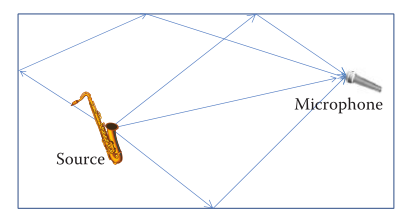
\includegraphics[scale=0.5]{./figuras/reverb01.png}
			\caption{Ilustração do efeito de Reverberação.}
			\label{reverb01}
		\end{figure}
		
		Muito embora possa parecer ao primeiro momento, o efeito de reverberação é muito mais que uma série de ecos. Um eco, por exemplo, pode ser entendido um resultado de uma distinção, atraso de versões de um som, o qual você pode ouvir com um atraso no mínimo de 40 milissegundos. Já a reverberação de uma sala vazia, por exemplo, há muitas e muitas reflexões, e as primeiras delas que chegam ao receptor são muito mais curtas que termos de tempo de duração. Logo essas reflexões não são tão percebidas ou distinguidas do som da fonte diretamente. Em vez disso, nós percebemos apenas o efeito da combinação de todas essas reflexões.
		
		\begin{figure}[!ht]
			\centering
			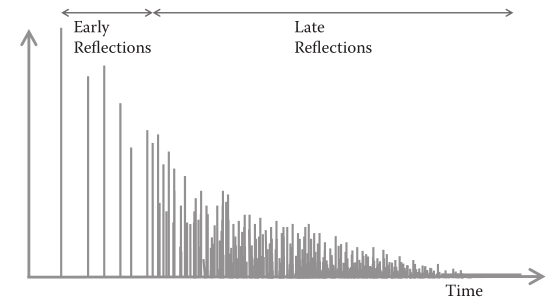
\includegraphics[scale=0.5]{./figuras/reverb02.png}
			\caption{Resposta de um Impulso de uma sala pequena.}
			\label{reverb02}
		\end{figure}
		
		Nesse sentido, podemos também considerar que a reverberação do som é mais do que um simples dispositivo de \textit{delay} com retorno. No \textit{reverb} a taxa em que as reflexões chegarão muda ao longo do tempo, em oposição de termos apenas que simular reflexões que tenham um intervalo fixo entre elas. Essas reflexões são relacionadas a posição do som que o receptor está na sala, ao tipo de construção da sala (oval, retangular), tamanho e material das paredes. 
		
		
	\subsection{Tipos de Reverb}
	
		Efeitos de \textit{reverb} são alcançados pela utilização de uma série complexa de \textit{delays} de um mesmo sinal que diminuem em amplitude e clareza de modo a simular o comportamento acústico de um espaço real. Falando sob o aspecto musical e industrial de equipamentos que realizam o processamento e simulação de efeitos de repetição (tal como o reverb, delay) termos no mercado diversos tipos de \textit{reverb`s}, os quais possuem diferentes aplicações que veremos a seguir:
		
		\begin{itemize}
			\item \textbf{Spring} ("Reverb-de-mola") - O efeito de reverberação com mola é um método que foi primeiramente proposto por \textit{Hammond} em 1940s. O reverb de mola foi criado naturalmente, por um sistema mecânico, o qual usa um transdutor e um captador nas extremidades de uma mola, para criar e capturar vibrações dentro dela. Muitos amplificadores de guitarra incluem esse tipo de reverberação dentro de seus projetos. Existem ainda muitos pedais de reverb que oferecem esse efeito emulado digitalmente e apenas algumas companhias, por questões de custo de construção, também lançaram produtos com um sistema real de reverb de molas.
			
			\begin{figure}[!h]
				\centering
				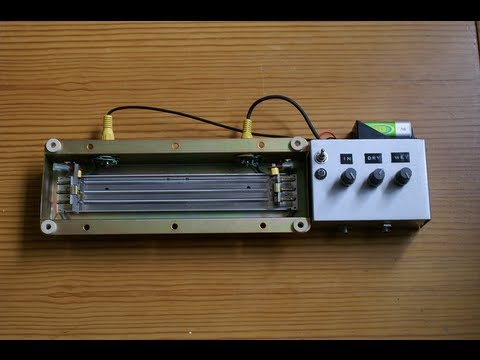
\includegraphics[scale=0.3]{./figuras/spring-reverb.jpg}
				\caption{Câmara de reverb de mola de um amplificador}
				\label{spring-reverb}
			\end{figure}
			
			\item \textbf{Room} ("Reverb-sala") - Este tipo de reverb é usado para simular um som natural de uma sala acústica, geralmente vazia, que tem um tamanho geralmente pequeno. Esses reverbs usualmente possuem reflexões curtas que desaparecem rapidamente com o tempo. 
			
			\item \textbf{Hall} ("Reverb-palco") - Reverb's dessa categoria são usados para simular um tipo de reverberação encontrado num grande teatro ou até mesmo catedrais ou igrejas. Eles "soam" geralmente mais fortes do que um \textit{room reverb} por conta da quantidade de reflexões serem significativamente maiores e mais longas. Pode ser encontrado a variação de hall reverbs como "\textit{cathedral}".
			
			\item \textbf{Plate} ("Reverb-de-placas") - Um plate reverb é definitivamente o efeito que exige uma grande logística a ser empregada. Uma grande máquina conforme mostrado na figura () a qual fornece o áudio dentro de grandes "placas" penduradas de metal que produzem um som de reverb que é mais definido do que o efeito do hall-reverb enquanto ainda é capaz de produzir longos decaimentos no tempo.
			
			\begin{figure}[!h]
				\centering
				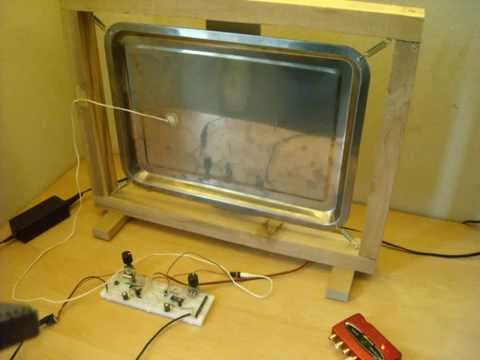
\includegraphics[scale=0.3]{./figuras/plate-reverb.jpg}
				\caption{Pequeno protótipo de um reverb de placas.}
			\end{figure}
			
			\item \textbf{Pitch-Shifter Reverb} aka \textbf{Shimmer} - Bem esse efeito de reverb será o foco de desenvolvimento desse trabalho. O shimmer tem se tornado bem comum entre pedais de guitarra principalmente nesses últimos anos. A grosso modo, esses reverbs adicionam componentes harmônicos do som original para dar a sensação de ambiência e harmonia e simulam a reverberação desses sons mais agudos na "cauda" (no final do reverb).
			
			Este som tem características bem peculiares, as quais geralmente as pessoas associam a um som de orquestra angelical ou sintetizadores de teclado, dando uma intensa ambiência e atmosfera no som.
			
			Diferente dos demais reverbs, o Shimmer é um efeito eminentemente sintetizado, ou seja, produzido digitalmente por meio de algoritmos embarcados em DSP`s e comercializados como equipamentos de produção digital.
			
		\end{itemize}
	
	\subsection{Pitch Shifting}
	
		\subsubsection{Conceitos Inicias}
		
			Entre os efeitos digitais de áudio (especialmente os realizados em tempo real), esse é um dos que exige algoritmos mais sofisticados, e até recentemente, os resultados não eram convincentes. 
			
			A primeira consideração a ser feita sobre esse assunto seria entender o que é um \textit{pitch shifting}. A melhor definição para o termo "pitch"de um som seria o conjunto de frequências de que o som é formado. A melhor maneira de entender esta definição é olhar por exemplo um coral. Nele há tanto mulheres quanto homens cantando mas as mulheres tem um "alcance"/pitch mais alto que o homem. A mudança das frequências masculinas, por exemplo, para frequências mais altas, o faria
			parecer como uma voz feminina.
			
			O efeito funciona comprimindo e, posteriormente expandindo o sinal que está sendo processado. A grosso modo, para transpor um som uma frequência mais acima, o sinal é tocado mais rápido, o que o torna mais curto. Então é preciso copiar segmentos do sinal processado e adicioná-lo ao sinal resultante para eliminar essa diferença temporal. 
			
			Para tornar um som mais grave, o sinal é reproduzido mais lentamente, o que requer o corte de algumas seções do sinal para diminuir sua duração. Ou seja, \textit{pitch shifters} estão constantemente cortando ou colando pequenas porções do áudio a ser processado.
			
		\subsubsection{Escala de Frequência Musical - \textit{Pitch Shift}}
			É sabido que a escala musical é dividida em várias oitavas. Cada oitava é composta por 12 (doze) semitons, também são referenciados como meio salto.
			
			Cada nota corresponde a uma frequência fundamental que a compõe. Essa frequência é definida pela equação \ref{eq-escala01}, onde $ p $ corresponde ao número de semitons e $ f $ a frequência em Hertz.
			
			\begin{equation}
				\label{eq-escala01}
				p = 69 + 12.\log(f/440)
				\caption{Equação que relaciona os semitons com a frequência fundamental}
			\end{equation}
			
			Sob a óptica de sinais e sistemas, um pitch shifting consiste em deslocar a frequência fundamental e suas harmônicas por um fator específico, conforme mostrado na equação (). A equação consiste na obtenção da frequência final $f_{final}$ dado a frequência inicial $ f_{inicial} $, e os números de semitons "$ s $" os quais pretende deslocar.
			
			\begin{equation}
				\label{eq-escala02}
				f_{final} = 2^{(s/12)}.f_{inicial}
			\end{equation}
			
			Como já mencionado, existem 12 semitons por oitava. Isso implica que cada transposição para cima ou para baixo uma oitava é equivalente na escala do espectro a multiplicar por 2 ou 1/2 respectivamente. A figura () ilustra as componentes de frequência (com um fator de $2^{(4/12)}$) o qual equivale a um \textit{pitch shift} de 4 semitons acima (de C para E).
						
\section{Comparativo entre soluções de Hardware}
		
		De acordo com a seção \ref{aplicabilidade}, numa sala de concerto, o som que espectador ouve contém tanto o som original produzido pela fonte (voz, instrumento acústico, sistema de sonorização, etc) quanto às milhares de reflexões desse som original, que bate no chão, paredes e teto, até chegar aos ouvidos, com um pequeno atraso. Essas reflexões são como milhares de ecos do sinal direto que, devido à sua grande quantidade, não são percebidas exatamente como ecos, mas sim como o efeito de “reverberação”. 
		
		Baseados na reflexividade de um ambiente podemos distinguir os materiais de que ele é composto. Em salas grandes com paredes elevadas de tijolo a reverberação geralmente é muito pesada e precisa de algum tempo até cessar. Já uma sala pequena, com muitos objetos dentro, possui uma reverberação muito pequena, em geral nem percebida como tal. Entretanto, essa pequena reverberação de fato existe, e por essa a razão é que os projetistas de processadores de efeitos incluírem vários tipos básicos de reverberações, dando a eles nomes de tipos diferentes de “salas” - room reverb. É muito natural, por exemplo, que uma programação de reverb chamada “Catedral” - reverb hall produza uma reverberação longa e muito densa, enquanto uma programação chamada de “Room” represente a acústica de uma sala muito menor \cite{Albar2007}. 
		
		Diante dessa realidade, no mercado, atualmente, várias são as empresas que possuem em seu portfólio esse tipo de efeito com essas características clássicas. Contudo, o efeito \textit{shimmer} é um dos mais complexos a serem implementados na prática devido ao seu alto custo de processamento. Todos os detalhes serão abordados mais a frente neste trabalho.
		
		\begin{mymdframed}{NOTA}
			Vale destacar que o efeito puramente de reverberação já é notoriamente conhecido e manipulado por diversos hardwares e softwares no mercado. Note-se que estamos falando do efeito adicional incorporado ao produto que é o chamado \textit{shimmer}.
		\end{mymdframed}
	
		\subsection{Hardwares de Reverb-Shimmer}
			
			Apesar dos equipamentos ora aqui listados serem conservacionalmente populares no meio musical, tendo diversas aplicações em projetos musicais, infelizmente não se pôde obter detalhes técnicos específicos, em termos de performance de \textit{hardware}, além do que consta em seus manuais ou algum \textit{review} na internet, os quais foram de imensa ajuda principalmente para o produto da empresa Strymon (\textit{BigSky Reverb}).
			
			
			\begin{enumerate}
				\item \textbf{Eventide H9}: A Eventide, Inc. (também conhecida anteriormente como Eventide \textit{Clock Works Inc}., ou hoje simplesmente como Eventide) é uma companhia de áudio, transmissões, comunicações e aviônica dos Estados Unidos cuja divisão de áudio produz processadores de áudio, software DSP e efeitos de guitarra.
				Eventide foi uma das primeiras companhias a produzir processadores de áudio digital e seus produtos são fundamentais em gravação e reprodução de som, pós-produção e estúdios de transmissão. Ela possui um pedal de guitarra chamado H9 (\ref{eventide-h9}) "revolucionário" que embarca diversos tipos de efeito e possui grande poder de processamento e efeito com qualidade profissional num formato relativamente compacto. Neste pedal é possível importar algoritmos de efeitos de modulação, de repetição e diversas ambiências tal como o efeito de reverb shimmer tudo através de sua entrada serial universal (USB) utilizando um \textit{software} proprietário.
				
				\begin{figure}[!h]
					\centering
					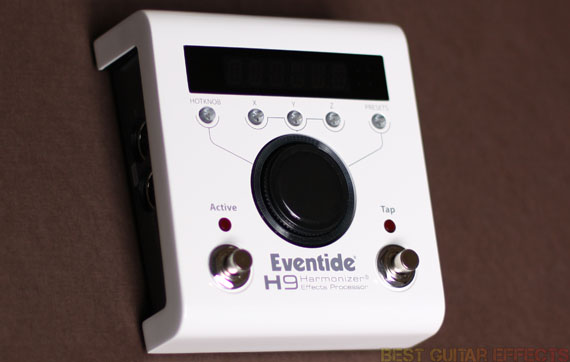
\includegraphics[scale=0.3]{./figuras/eventide-h9.jpg}
					\caption{Foto modelo Eventide H9 - Effects Processor.}
					\label{eventide-h9}
				\end{figure}
				
				\item \textbf{Strymon BigSky}: A empresa Strymon, fundada em meados de 2008, é considerada uma das empresas mais bem sucedidas no universos de pedais de guitarra de linha exclusiva (\textit{boutique-pedals}) que integram algoritmos de tratamento de sinais de áudio extremamente avançados.
				
				Vale salientar que com tantas grandes empresas produzindo diversos produtos, sendo por vezes um réplica do outro, é impressionante ver uma pequena empresa produzir um produto de qualidade notoriamente alta. Foi, de fato, uma reinvenção da roda em termos de qualidade dos efeitos e o resultado esperado pelo usuário final.
				
				\begin{enumerate}
					\item \textbf{Qualidade de Áudio}: \begin{itemize}
						\item Baixo ruído na entrada do dispositivo, alta peformance de aúdio com resolução de 24-bit  e taxa de amostragem de 96kHz, tanto para o conversor Analógico digital quanto para o conversor digital analógico.
						\item 115 db de relação sinal-ruído em 50% de wet mix ou 
					\end{itemize}
					
					\item \textbf{Processador}:
				\end{enumerate}
				
				
				 
			\end{enumerate} 
		
	\subsection{Micontroladores e DSP's}

		O termo sistemas embarcados constituem circuitos eletrônicos que utilizam processadores digitais (microprocessadores ou microcontroladores, etc.) em aplicações dedicadas para determinado equipamento ou produtos.
		
		Os microcontroladores, diferentemente dos microprocessadores, em geral, possuem todos os periféricos necessários num único chip. Seu tamanho também é muito pequeno, mesmo contendo vários periféricos como: memórias, barramentos, \textit{timers}, portas de comunição, conversores de sinal analógicos para digital etc.
		
		Por outro lado, esses dispositivos possuem um desempenho menor que os microprocessadores, mas são ideais em aplicações que necessitam de menores dimensões, tempo e custos.
		
		As linguagens de programação das unidades processadores de sistemas embarcados podem variar, mas em geral, se limitam às linguagens C/C++, \textit{Assembly} e \textit{Java}.
		
		Nessa linha, temos ainda o processador digital de sinais (DSP - \textit{Digital Signal Processing}) e pode definir tanto o processador quanto o processo em si. Esse tipo de tratamento exige um alto desempenho para aplicações numéricas em tempo real.
		
		Os DSP's são construídos para computar de forma eficiente equações de diferenças e algoritmos de transformadas diversas (como a \textit{Fast Fourier Transform} - FFT). As aplicações dos DSP's, em suma, estão relacionadas com sistemas de controle de alta velcodiade, realizações de filtros digitais, transformadas rápidas de \textit{Fourier}, processamento de sons e imagens, entre outras.

	\subsection{Hardwares Comerciais do Efeito \textit{Reverb - Shimmer}}
	
	\subsection{Microcontrolador MSP430F5529 e TMS320}
	
	Foram utilizados ao longo do projeto como soluções de hardware essencialmente o \textit{microntrolador launchpad MSP430F5529}.
	
	Não obstante foram apontados na subseção anterior a respeito das limitações do hardware para tratamento de sinais de áudio em tempo real, o escopo do trabalho levou em consideração a economicidade do hardware em questão, bem como a utilização de operações no domínio do tempo, sem utilização de etapas intermediárias como realização da transformada de \textit{Fourier} para manipulação do sinal de áudio. %melhorar esse texto
	
	Além disso, o projeto teve uma participação do desempenho do TSM320 C2000 o qual, devido ao tempo de aprendizagem do DSP para correta aplicabilidade no projeto, não fora possível. %melhorar o texto


\section{Objetivos e Diagrama de Bloco do Projeto}

	Nosso objetivo neste trabalho é o estudo e a realização de um projeto, desenvolvido em \textit{software} e futuramente aplicado em \textit{hardware}, de um efeito digital de aúdio seletivo em frequência que tem como característica musical a repetição assíncrona do som (reverb) com destaque na utilização de componentes de frequências (harmonicas) na realização desse efeito (\textit{shimmer}).
	
	Nesta parte do trabalho, será mostrado de maneira abstrata os blocos necessários para que obtenha a saída do sistema desejado , ou seja, o efeito do \textit{Reverb} com \textit{Shimmer} implementado em software e executado seja em software ou em hardware.
		
	Temos aqui na figura \ref{bloco-principal} um sinal analógico oriundo e um instrumento musical - guitarra, que passa por um processador de som digital - DSP, o qual procede com todo o trabalho tratamento desse sinal analógico ora convertido amostras digitais. Aplicando, portanto, nesse contexto, um filtro de resposta finita; um algoritmo de seleção de frequências denominado \textit{pitch-shifter} e por fim realimentando o sistema acrescentando um pequeno atraso temporal (\textit{delay}).
	
	\begin{figure}[!h t b]
		\centering
		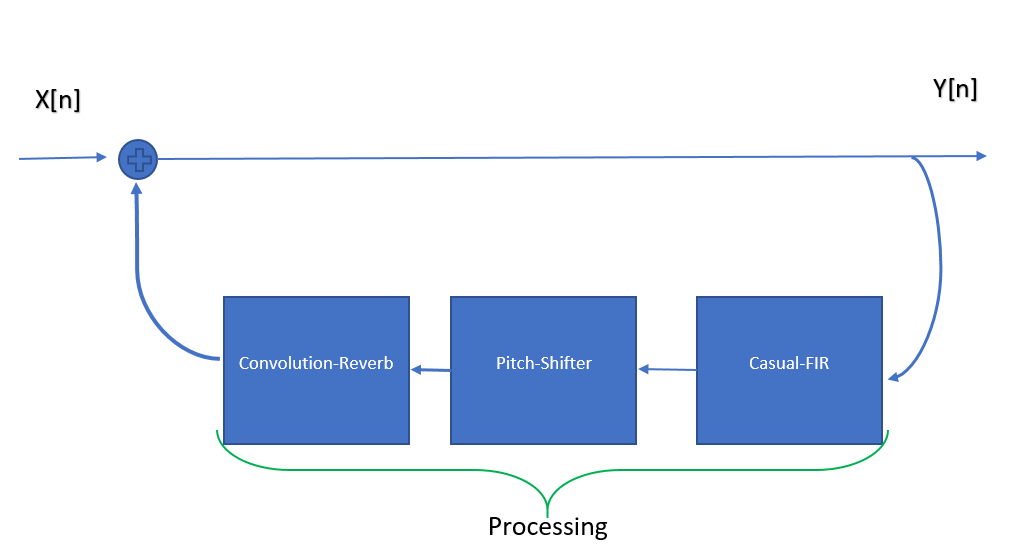
\includegraphics[scale=0.5]{./figuras/diagrama_bloco_principal.PNG}
		\caption{Diagrama de Blocos Principal do Projeto.}
		\label{bloco-principal}
	\end{figure}
	

%	----------------------------------
	Como uma lei de controle de malha fechada podemos ilustrar (figura \ref{signal_principal}) também como um diagrama de fluxo de sinais da seguinte forma:
	
	\begin{figure}[!h t b]
		\centering
		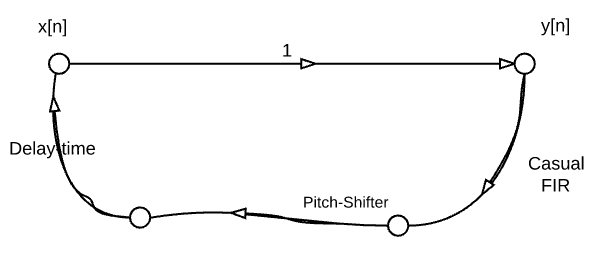
\includegraphics[scale=0.5]{./figuras/fluxo_de_sinais_principal.png}
		\caption{Diagrama de Fluxo de Sinais do Projeto.}	
		\label{signal_principal}
	\end{figure}
	
	Não obstante ao modelo apresentado, também será objeto de estudo os blocos que compõe a conversão do sinal analógico para a realidade de amostras digitais (conversão A/D), bem como o caminho inverso que propõe o envio das amostras a um conversor gerador de níveis de tensão elétrica correspondente (conversão D/A).
	
	
	
	
	


\chapter{Metodologia e Ferramentas}


\section{Sinais de Tempo Discreto e Transformada Discreta de \textit{Fourier}}

\section{Filtros Digitais}

	\subsection{Conceitos Iniciais}
	
		Os filtros digitais não contém uma implementação física em si, diferentemente dos filtros analógicos constituídos, geralmente, de associação de resistores e capacitores. Eles são construídos através de algoritmos.
		
		Para que isso possa ocorrer é necessário que o sinal de áudio (analógico) seja devidamente convertido em um sinal digital. esse sinal portanto convolui por um algoritmo de filtro adequado.
		
		De maneira geral, o projeto de um filtro consite em obter os coeficientes para os filtros. Isso é realizado através de uma equação chamada de equação das diferenças. O processo pode ser simplesmente realizado pela equação (\ref{eq-filtro-bas}):
		
		\begin{equation}
			\text{Saida} = \sum_{1}^{n} \text{Coeficiente}_n \text{do filtro} * \text{Amostra}_n
			\label{eq-filtro-bas}
		\end{equation}
		
		Assim, o contexto de um filtro digital estará associado a equações de diferenças (ou funções de transferência no domínio Z) cujo parâmetros (coeficientes) serão calculados com o objetivo de discriminar (extrair, atenuar, etc.) determinadas componentes espectrais presentes em um sinal ou uma informação no mesmo sentido dos filtros analógicos, sem a necessidade de um circuito (\textit{hardware}) adicional. Em outras palavras, o filtro digital será uma rotina adicional agregada ao algoritmo responsável pela realização do sistema proposto em questão.
		
	\subsection{Filtros IIR}
		
		Os filtros digitais de resposta infinita ao impulso (\textit{Infinite Impulse Response - IIR}), também conhecidos como filtros recursivos ou autorregressivos, são modelados pela equação de diferença (\ref{eq1-iir}) ou pela função de transferência (\ref{eq2-iir-tf}), em que basicamente os valores dos coeficientes dos modelos define a natureza do filtro (passa-baixa; passa-alta; passa-faixa; rejeita-faixa).
		
		A denominação de IIR se deve que a saída do modelo decai para um valor nulo em um tempo infinito em resposta a um impulso aplicado na entrada filtro correspondente.
		
		\begin{equation}
			y(k) = \frac{1}{a_0}\left(\sum_{m=0}^{M}b_mx(k-m)-\sum_{n=1}^{N} a_ny(k-n)\right)
			\label{eq1-iir}
		\end{equation}
		
		\begin{equation}
			D(z) = \frac{y(z)}{x(z)} = \frac{b_0 + b_1z^{-1}+...+ b_mz^{-m}}{a_1z^{-1}+ a_nz^{-n}}
			\label{eq2-iir-tf}
		\end{equation}
		
		Resumidamente, a forma usual de calcular os coeficientes de um filtro digital IIR consiste em utilizar o modelo de um filtro analógico, e aplicar uma transformada Z via aproximação retangular ou trapezoidal \cite{Schlichthaerle2011}.
		
		Notoriamente, uma das vantagens na utilizacão dos filtros IIR é que eles resultam em comprimentos (quantidade de coeficientes) de filtro menor do que o filtro FIR correspondente, porém, esta melhoria é obtida às custas de distorção de fase e um transitório que não se limita a um intervalo de tempo finito \cite{Haykin1999}.
		
		
	\subsection{Filtros FIR}
	
		\
		
		
	
	
	\subsection{Filtros Adaptativos}
		Os filtros adaptativos são constituídos, geralmente, por estruturas FIR, em que os coeficientes dos modelos associados são modificados conforme um procedimento adaptativo. essa modalidade de filtro geralmente é empregada nos seguintes contextos (\textit{lista não exaustiva}):
		
		\begin{itemize}
			\item Como procedimento alternativo na obtenção de valores dos coeficientes de um determinado filtro FIR, em que padrões de entrada e saída conhecidos são utilizados para estabelecer os valores dos coeficientes do filtro em questão;
			\item Cancelamento ou redução de ecos/barulhos de um determinado ambiente;
			\item Na modelagem de sistemas dinâmicos; e
			\item Como modelagem básica de representações de redes neurais artificiais.
		\end{itemize}
	
		A equação () representa o modelo de um filtro FIR, em que $W_m(k)$ denota os valores dos coeficientes do filtro em um instante de tempo $k$. 
		
		\begin{equation}
			\label{eq1-filtroadap}
			y(k) = \sum_{m=0}^{M} W_m(k)x(k-m)
		\end{equation}
		
		A diferença ou erro $\epsilon(k)$ entre o valor de padrão desejado d(k) para a a resposta do filtro e a informação da saída atual $y(k)$ do modelo associado é expressa por:
		
		\begin{equation}
			\label{eq2-filtroadap}
			\epsilon(k) = d(k)- y(k)
		\end{equation}
		
		Basicamente para ajustar os valores dos coeficientes de um filtro adaptativo tipicamente utiliza o método do gradiente para essa finalidade (fonte....), sendo o critério da somatória do erro quadrático de $\epsilon_(k)$ frequentemente utilizado na etapa de adaptação.
		
		Vale salientar, que alguns sistemas de comunicação de voz utilizam filtros adaptativos com o objetivo de cancelar ou reduzir ecos ou barulhos do ambiente. Nesse contexto, foi pensado inicialmente a utilização desse modelo de filtro para o projeto. No entanto, será explicado mais a frente a não adoção desse modelo, bem como pela utilização de um filtro FIR típico.
		
		
\section{Ferramentas Computacionais}
\chapter{Implementação do Projeto}

\section{Bloco 0 - Conversão Analógico Digital}

\section{Bloco 1 - Projetando um Filtro FIR}
	\subsection{Microntrolador MSP 430}
		Aqui será dada uma pequena atenção a respeito da escolha do microcontrolador da \textit{Texas Instruments} para o referido projeto, em especial as vantagens auferidas:
		
		\begin{enumerate}
			\item Baixo Consumo:
			\item Baixa Tensão de Operação:
			\item Alta Performance:
			\item Grande Quantidade de Periféricos:
		\end{enumerate}
	\subsection{Comunicação Serial}
		

\section{Bloco 2 - Implementando o Pitch-Shifter}

\section{Bloco 3 - Delay Time}
\chapter{Simulações e resultados}
	Neste capítulo, serão apresentados os resultados experimentais de todo o processo de obtenção do efeito de \textit{Reverb Shimmer}, bem como alguns resultados de testes de pequenos algortimos implementados no microcontrolador MSP430F5529 com seu conversor Analógico Digital de 12 bits e a comunicação I$ ^2 $C entre o $ \mu C $ e o dispositivo MCP 4725.
	
	Os experimentos ora mostrados foram realizados de forma a demonstrar toda a abordagem de aprendizagem durante o projeto. Conforme será explicado na conclusão do trabalho, posto que foi identificado, através de experimento e cálculos realizados na implementação as limitações do hardware proposto para a execução do código do efeito digital em si.

	\section{Descrição dos Experimentos}
		
		Os resultados das simulações serão divididos da seguinte ordem:
		
		\begin{enumerate}
			\item Comparativo da quantização de um sinal de aúdio com resoluções de 16 e 12 bits;
			\item Comparativo da quantização de um sinal de aúdio com resoluções de 12, 10 e 8 bits;
			\item 
		\end{enumerate}
	
		Para os experimentos acima mencionados serão utilizados os seguintes dados mostrado na tabela ():
		
		\begin{tabular}[ht!]{|c|c|}
			\hline 
			Fonte de Áudio		&	\textit{'guitar-clean16.wav'} - som de guitarra limpa\\
			\hline
			Taxa de Amostragem 	&	44100 Hz	\\
			\hline
			Número de Canais 	&	1 canal mono\\ 
			\hline

		\end{tabular}
		
		
		\begin{figure}[!ht]
			\label{fig-exp1}
			\centering
			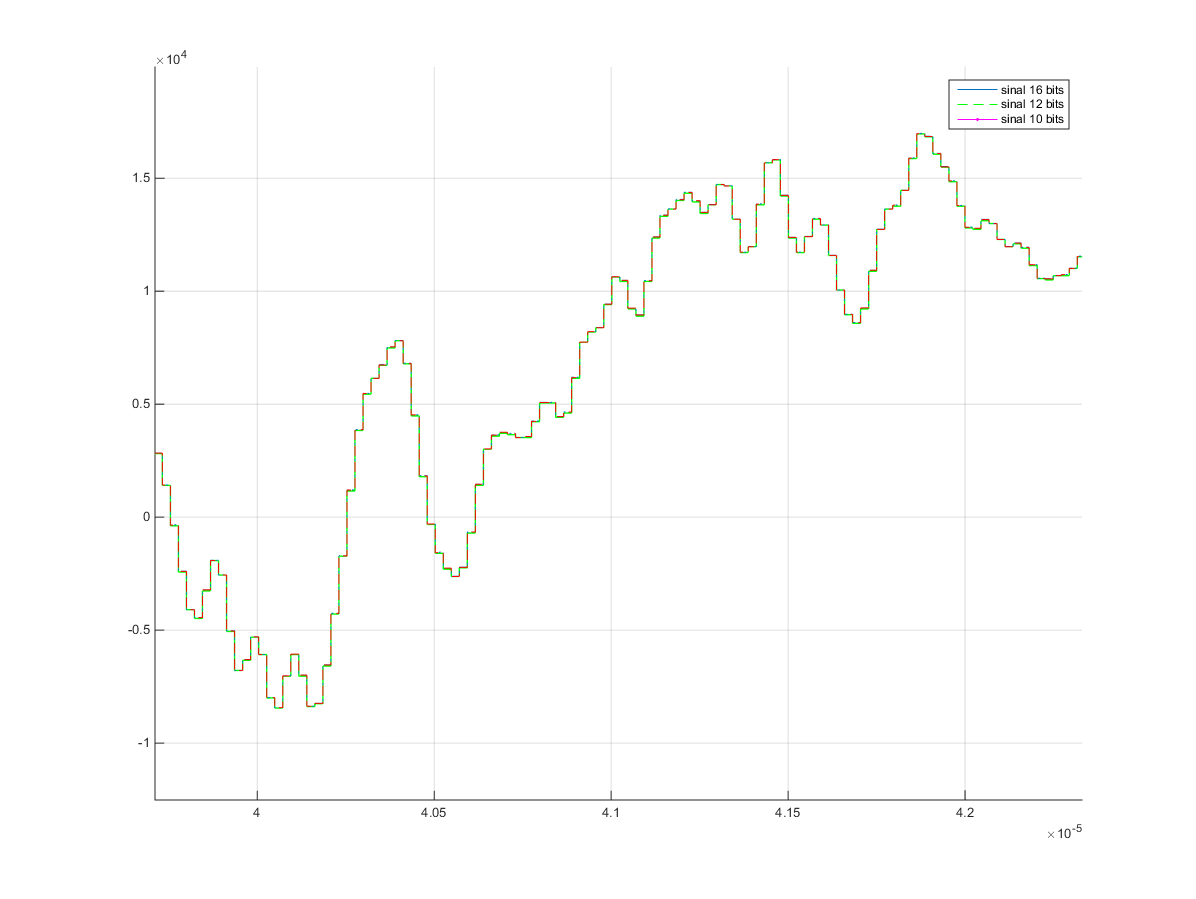
\includegraphics[scale=0.5]{./figuras/simulacoes/resolucao-audios/10-12-16-normal.png}
			\caption{Quantização do sinal de áudio em 10, 12 e 16 bits PCM}
		\end{figure}
		
		\begin{figure}[!ht]
			\label{fig-exp2}
			\centering
			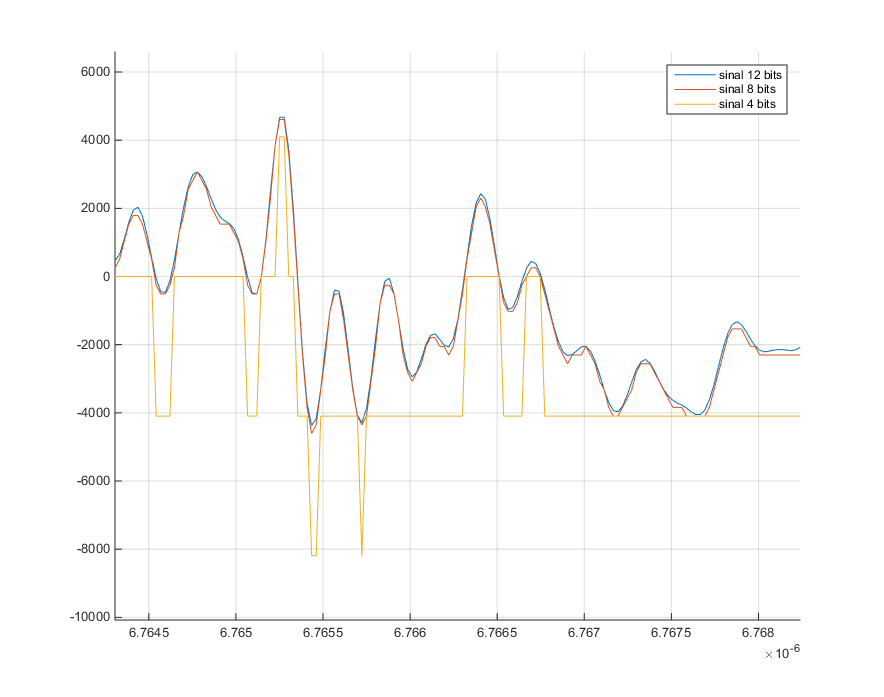
\includegraphics[scale=0.5]{./figuras/simulacoes/resolucao-audios/12-8-4-normal.png}
			\caption{Quantização do sinal de áudio em 12, 8 e 4 bits PCM}
		\end{figure}
	
		Esses resultados das figuras  são apenas a título de informações preliminares na escolha da resolução adequada para que o sinal seja tratado posteriormente no microcontrolador. Nesse caso, posto que o conversor em questão seja de 12 (doze) \textit{bits} percebe-se que não há uma perda significativa na resolução do sinal, bem como audivelmente não se percebeu grande perda de qualidade em relação ao áudio original em 16 \textit{bits}.
	
		
	
	


\chapter{Conclusões}

 			
	\section{Realização do Projeto}
	\label{realizacao-projeto}
		O projeto foi executado dentro das limitações impostas de hardware do uC MSP430F5529LP no quesito de seu desempenho de conversão digital analógica, bem como suas interrupções, período de amostragem bem como sua integração com o conversor Digital-Analógico MCP4725 através da interface $ I^2C $.
		
		Não foram avaliados, no entanto, o desempenho do dispositivo na aplicação dos filtros digitais e o modelo ora projetado no \textit{software} Matlab que demonstrou o efeito de \textit{reverb-shimmer} em si. Muito embora, essa parte do projeto estivesse dentro do escopo inicial do trabalho, a sua realização se daria com melhores resultados com a utilização de um DSP específico para esta aplicação, nesse caso a utilização do TMS320F2837xS $\text{Delfino}^{TM}$.
		
		Foram constatados que o efeito \textit{reverb-shimmer} possui uma grande complexidade em termos de estabilidade, pois, conforme observado nas simulações, a malha de realimentação com o bloco de \textit{delay`s} aleatórios podem deixar o sistema instável e com isso efeitos indesejados no resultado final.
		
		Dentro dessa realidade podemos dizer que o objetivo do trabalho foi alcançado com respeito ao entendimento claro do modelo matemático e suas implicações na escolha de se projetar um efeito seletivo em frequência, entender suas limitações dentro do contexto de filtros digitais, seu critério de estabilidade e consubstanciar elementos necessários para que seja aplicado dentro de um contexto de projeto de \textit{hardware}.
	
	\section{Auto-Crítica}
		Considerando a seção \ref{realizacao-projeto}, vale destacar, por ora, que a realização em hardware foi a maior dificuldade encontrada dentro do projeto por conta das escolhas dos parâmetros limitantes, tais como:
		
		\begin{enumerate}
			\item Resolução da conversão - 12 bits;
			\item Período de Amostragem do \textit{Timer};
			\item Imprecisão nas amostras coletadas;
			\item Impossibilidade de trabalhar com ponto flutuante.
		\end{enumerate}
		
		Diante disso foi necessário concluir o trabalho apenas entendendo as limitações de hardware e escolhendo seus parâmetros baseado nos conceitos de processamento digitais de sinais e não apenas em testes cegos de desempenho. Por outro lado, não se avaliou o desempenho com os códigos ora projetados no MATLAB para o uC em questão, mesmo este sendo o modelo mais modesto.
		
	\section{Modelos para Trabalhos Futuros}
	

%\chapter{Metodologia e Ferramentas}


\section{Sinais de Tempo Discreto e Transformada Discreta de \textit{Fourier}}

\section{Filtros Digitais}

	\subsection{Conceitos Iniciais}
	
		Os filtros digitais não contém uma implementação física em si, diferentemente dos filtros analógicos constituídos, geralmente, de associação de resistores e capacitores. Eles são construídos através de algoritmos.
		
		Para que isso possa ocorrer é necessário que o sinal de áudio (analógico) seja devidamente convertido em um sinal digital. esse sinal portanto convolui por um algoritmo de filtro adequado.
		
		De maneira geral, o projeto de um filtro consite em obter os coeficientes para os filtros. Isso é realizado através de uma equação chamada de equação das diferenças. O processo pode ser simplesmente realizado pela equação (\ref{eq-filtro-bas}):
		
		\begin{equation}
			\text{Saida} = \sum_{1}^{n} \text{Coeficiente}_n \text{do filtro} * \text{Amostra}_n
			\label{eq-filtro-bas}
		\end{equation}
		
		Assim, o contexto de um filtro digital estará associado a equações de diferenças (ou funções de transferência no domínio Z) cujo parâmetros (coeficientes) serão calculados com o objetivo de discriminar (extrair, atenuar, etc.) determinadas componentes espectrais presentes em um sinal ou uma informação no mesmo sentido dos filtros analógicos, sem a necessidade de um circuito (\textit{hardware}) adicional. Em outras palavras, o filtro digital será uma rotina adicional agregada ao algoritmo responsável pela realização do sistema proposto em questão.
		
	\subsection{Filtros IIR}
		
		Os filtros digitais de resposta infinita ao impulso (\textit{Infinite Impulse Response - IIR}), também conhecidos como filtros recursivos ou autorregressivos, são modelados pela equação de diferença (\ref{eq1-iir}) ou pela função de transferência (\ref{eq2-iir-tf}), em que basicamente os valores dos coeficientes dos modelos define a natureza do filtro (passa-baixa; passa-alta; passa-faixa; rejeita-faixa).
		
		A denominação de IIR se deve que a saída do modelo decai para um valor nulo em um tempo infinito em resposta a um impulso aplicado na entrada filtro correspondente.
		
		\begin{equation}
			y(k) = \frac{1}{a_0}\left(\sum_{m=0}^{M}b_mx(k-m)-\sum_{n=1}^{N} a_ny(k-n)\right)
			\label{eq1-iir}
		\end{equation}
		
		\begin{equation}
			D(z) = \frac{y(z)}{x(z)} = \frac{b_0 + b_1z^{-1}+...+ b_mz^{-m}}{a_1z^{-1}+ a_nz^{-n}}
			\label{eq2-iir-tf}
		\end{equation}
		
		Resumidamente, a forma usual de calcular os coeficientes de um filtro digital IIR consiste em utilizar o modelo de um filtro analógico, e aplicar uma transformada Z via aproximação retangular ou trapezoidal \cite{Schlichthaerle2011}.
		
		Notoriamente, uma das vantagens na utilizacão dos filtros IIR é que eles resultam em comprimentos (quantidade de coeficientes) de filtro menor do que o filtro FIR correspondente, porém, esta melhoria é obtida às custas de distorção de fase e um transitório que não se limita a um intervalo de tempo finito \cite{Haykin1999}.
		
		
	\subsection{Filtros FIR}
	
		\
		
		
	
	
	\subsection{Filtros Adaptativos}
		Os filtros adaptativos são constituídos, geralmente, por estruturas FIR, em que os coeficientes dos modelos associados são modificados conforme um procedimento adaptativo. essa modalidade de filtro geralmente é empregada nos seguintes contextos (\textit{lista não exaustiva}):
		
		\begin{itemize}
			\item Como procedimento alternativo na obtenção de valores dos coeficientes de um determinado filtro FIR, em que padrões de entrada e saída conhecidos são utilizados para estabelecer os valores dos coeficientes do filtro em questão;
			\item Cancelamento ou redução de ecos/barulhos de um determinado ambiente;
			\item Na modelagem de sistemas dinâmicos; e
			\item Como modelagem básica de representações de redes neurais artificiais.
		\end{itemize}
	
		A equação () representa o modelo de um filtro FIR, em que $W_m(k)$ denota os valores dos coeficientes do filtro em um instante de tempo $k$. 
		
		\begin{equation}
			\label{eq1-filtroadap}
			y(k) = \sum_{m=0}^{M} W_m(k)x(k-m)
		\end{equation}
		
		A diferença ou erro $\epsilon(k)$ entre o valor de padrão desejado d(k) para a a resposta do filtro e a informação da saída atual $y(k)$ do modelo associado é expressa por:
		
		\begin{equation}
			\label{eq2-filtroadap}
			\epsilon(k) = d(k)- y(k)
		\end{equation}
		
		Basicamente para ajustar os valores dos coeficientes de um filtro adaptativo tipicamente utiliza o método do gradiente para essa finalidade (fonte....), sendo o critério da somatória do erro quadrático de $\epsilon_(k)$ frequentemente utilizado na etapa de adaptação.
		
		Vale salientar, que alguns sistemas de comunicação de voz utilizam filtros adaptativos com o objetivo de cancelar ou reduzir ecos ou barulhos do ambiente. Nesse contexto, foi pensado inicialmente a utilização desse modelo de filtro para o projeto. No entanto, será explicado mais a frente a não adoção desse modelo, bem como pela utilização de um filtro FIR típico.
		
		
\section{Ferramentas Computacionais}
% etc

%%%%%%%%%%%%%%%%%%%%%%%%%%%%%%%%%%%%%%%%%%%%%%%%%%%%%%%%%%%%%%%%%%%%%%%%%
% Referências bibliográficas											%
%%%%%%%%%%%%%%%%%%%%%%%%%%%%%%%%%%%%%%%%%%%%%%%%%%%%%%%%%%%%%%%%%%%%%%%%%
%\bibliographystyle{config/abntex2/abntex2-num} % use este estilo para ABNT numérico
\bibliographystyle{config/abntex2/abntex2-alf} % use este estilo para ABNT numérico
\renewcommand{\bibname}{REFERÊNCIAS BIBLIOGRÁFICAS}
\phantomsection
\addcontentsline{toc}{chapter}{REFERÊNCIAS BIBLIOGRÁFICAS}
\bibliography{referencias}

%%%%%%%%%%%%%%%%%%%%%%%%%%%%%%%%%%%%%%%%%%%%%%%%%%%%%%%%%%%%%%%%%%%%%%%%%
% Anexos																%
%%%%%%%%%%%%%%%%%%%%%%%%%%%%%%%%%%%%%%%%%%%%%%%%%%%%%%%%%%%%%%%%%%%%%%%%%
\anexos
Code: "audio.m": Código MATLAB responsável pela realização do efeito shimmer numa amostra de Áudio:
\begin{lstlisting}
	clc;
	clear all;
	info = audioinfo('guitar.wav')
	[y,Fs] = audioread('guitar.wav','native');
	voiceL = y(1:1000000,1);
	%voiceR = y(:,2);
	
	for j = 1:15
	voiceL = [voiceL, bitshift(voiceL(:,j),-1)]; % shift once to the right
	%   voiceR = [voiceR, bitshift(voiceR(:,j),-1)];
	end
	
	voice = [voiceL];%todas as taxas de bits por amostras de 16bits ate 1
	%voice = voice/max(max(abs(voice)));
	
	output12bits = 2\^4.*voice(:,5);%coluna 5 da esquerda 12bits e 
	%coluna 20 do audio direito tbm
	%12bits
	output10bits = 2\^6.*voice(:,7);
	output8bits = 2\^8.*voice(:,9);
	output4bits = 2\^12.*voice(:,13);
	
	audiowrite('guitar12bits.wav',output12bits,info.SampleRate);
	audiowrite('guitar10bits.wav',output10bits,info.SampleRate);
	audiowrite('guitar8bits.wav',output8bits,info.SampleRate);
	audiowrite('guitar4bits.wav',output4bits,info.SampleRate);
	
	info = audioinfo('guitar12bits.wav')
	info = audioinfo('guitar10bits.wav')
	info = audioinfo('guitar8bits.wav')
	info = audioinfo('guitar4bits.wav')
	
	
	%Amostrando os sinais no tempo
	figure(1)
	hold on
	t = linspace(0,1/info.SampleRate,length(voice));
	plot(t,voice(:,1));%16 bits
	%plot(t,output12bits);%12 bits
	%plot(t,output10bits);%10 bits
	plot(t,output8bits);%8 bits
	%plot(t,output4bits);%4 bits
	legend('sinal 16 bits','sinal 8 bits');
	hold off;
	
	
	% comparacao valores maximos
	Max12bits = max(2\^4.*voice(:,5))
	Max16bits = max(voice(:,1))
	
	%amostrando o sinal no dominio da freq
	output12bits = double(output12bits);
	Y1 =    fft(output12bits);
	N = Fs;
	transform = fft(output12bits,N)/N;
	magtransform = abs(transform)/abs(max(abs(transform)));
	num_bits = length(magtransform);
	plot([0:1/(num_bits/2-1):1],magtransform(1:num_bits/2))
	% faxis = linspace(-Fs/2,Fs/2,N);
	% figure()
	% plot(faxis,magtransform);
	xlabel('frequency(Hz)')
	
	%projetar o filtro
	[b,a] = butter(8,0.1,'low');
	H = freqz(b,a,floor(num_bits/2));
	hold on
	figure()
	plot([0:1/(num_bits/2 -1):1], abs(H),'r');
	hold off
	figure()
	output12bits_filtrado = filter(b,a,output12bits);
	plot(output12bits,'b')
	hold on
	plot(output12bits_filtrado,'r')
	%normalizando
	output12bits_filtrado = output12bits_filtrado/max(abs(output12bits_filtrado));
	legend('audio 12 bits','audio 12bits filtrado');
	audiowrite('guitar12bitsfiltrado.wav',output12bits_filtrado,info.SampleRate);
	
	hold off
	%oitavador
	guitar_oitavado = pitchShift(output12bits,1024,256,2);
	guitar_oitavado_filter = filter(b,a,guitar_oitavado);
	
	%pequeno delay
	leftout=output12bits;  % set up a new array, same size as old one
	
	N=100;  % delay amount N/44100 seconds
	
	for n=N+1:length(guitar_oitavado_filter)
	
	leftout(n)=output12bits(n)' + guitar_oitavado_filter(n-N);  % approximately 1/4 second echo
	end
	output12bits = double(output12bits);
	Y1 =    fft(output12bits);
	N = Fs;
	transform = fft(output12bits,N)/N;
	magtransform1 = abs(transform)/abs(max(abs(transform)));
	num_bits = length(magtransform1);
	plot([0:1/(num_bits/2-1):1],magtransform1(1:num_bits/2))
	% faxis = linspace(-Fs/2,Fs/2,N);
	% figure()
	% plot(faxis,magtransform);
	hold on
	leftout = double(leftout);
	Y1 =    fft(leftout);
	N = Fs;
	transform = fft(leftout,N)/N;
	magtransform2 = abs(transform)/abs(max(abs(transform)));
	num_bits = length(magtransform2);
	plot([0:1/(num_bits/2-1):1],magtransform2(1:num_bits/2))
	% faxis = linspace(-Fs/2,Fs/2,N);
	% figure()
	% plot(faxis,magtransform);
	xlabel('frequency(Hz)')
	figure()
	plot(leftout)
	hold on
	plot(output12bits)
	legend('sinal de 12 bits','sinal com pitchshift+delay')
	leftout = leftout/max(abs(leftout));
	output12bits = output12bits/max(abs(output12bits));
	
	audiowrite('shimmerA.wav',leftout,44100)
\end{lstlisting}

Code: "mcp4725.c" - Cálculo do Conversor DAC de 12 bits. (amostragem Linear):
\begin{lstlisting}
	#include <msp430.h> 
	#include <stdint.h>
	#include "mcp4725.h"
	#include "lib/lcd/lcd.h"
	#include "lib/dma/dma.h"
	#include "lib/port/port.h"
	#include "lib/clock/clock.h"
	#include "lib/adc12/adc12.h"
	#include "lib/timers/timer.h"
	#include "lib/serial/serial.h"
	
	#define MCP4725 0x62
	#define mcpON      0
	#define mcpOFF1K   1
	#define mcpOFF100K 2
	#define mcpOFF500K 3
	
	uint16_t adcResult;
	uint16_t data = 0, write;
	
	int main(void) {
	watchDogStop();
	portInit();
	
	lcdInit();
	lcdClear();
	
	clockInit();
	clockSetDCO(1000000);
	clockSelect(DCO, SMCLK);
	clockSelect(DCO,  MCLK);
	
	adc12Init();
	portRoute2Perif(P6,0);
	
	//timerSetup(B0,ACLK,UP,3276,1000);
	TB0CTL   = TBSSEL__ACLK    |            // Select ACLK as clock source
	MC__UP          |            // Setup but do not count
	TBCLR;                       // Clear timer
	
	TB0CCR0  = 327;                        // Convert every 100ms
	TB0CCR1  = 100;                        // This can be anything
	TB0CCTL0 = CCIE;
	TB0CCTL1 = OUTMOD_3;                    // Set/reset
	
	dmaEnable(0);
	dmaTrgr(0,DMA_ADC12IFGx);
	dmaAddr(0,&ADC12MEM0,DMA_FIXED,&adcResult,DMA_FIXED);
	dmaMode(0,DMA_RPT_SINGLE_TRANSFER);
	dmaSize(0,1);
	
	serialInit(I2C);
	
	__enable_interrupt();
	
	//mcpWrite(0x2FF);
	
	volatile uint16_t recData[4096];
	uint16_t index = 4096;
	
	while(index) {
	while(!write);
	recData[--index] = adcResult;
	mcpWrite(index);
	write = 0;
	}
	while(1);
	}
	
	void mcpWrite(uint16_t data) {
	uint8_t vector[2];
	vector[0] = (data >> 8) & 0x0F;
	vector[1] = (data     ) & 0xFF;
	serialI2CSendData(MCP4725, vector, 2);
	}
	
	#pragma vector=TIMER0_B0_VECTOR
	__interrupt void isr_tb0_ccr0 () {
	write = 1;
	adcDisable();
	adcEnable();
	}
	
\end{lstlisting}

\makeatletter % não retirar estes comandos
\renewcommand{\@makechapterhead}[1]{%
  {\parindent \z@ \raggedleft \setfontarial\bfseries 
        \LARGE \thechapter. \space\space 
    \uppercase{#1}\par
    \vskip 40\p@
  }
}
\makeatother


% *** Anexo I: Diagramas esquemáticos ***
%\include{anexo_Codigosfonte}

%\refstepcounter{noAnexo}

% *** Anexo II: Descrição do CD ***
%\include{anexo_CD}
%\refstepcounter{noAnexo}

%\pdfbookmark[level]{text}{name}
% Acrescente mais anexos conforme julgar necessário.
\end{document}

